% The forecast timeline, from figures/forecast-timeline.mmd.
%
% The diagram itself is Mermaid; this file only places it and carries the
% caption and label, so \ref{fig:forecast-timeline} resolves the same way it
% did when the figure was drawn in TikZ.
%
% To regenerate after editing the .mmd:
%   cd docs/user-manual/figures
%   npx -y @mermaid-js/mermaid-cli -i forecast-timeline.mmd \
%       -o forecast-timeline.pdf -b white --pdfFit
% The PDF is vector, so it stays sharp at any print size.
%
% The TikZ original is still here as figures/forecast-timeline.tex. To go back,
% point content.tex at it instead of at this file -- nothing else changes.
\begin{figure}[htbp]
\centering
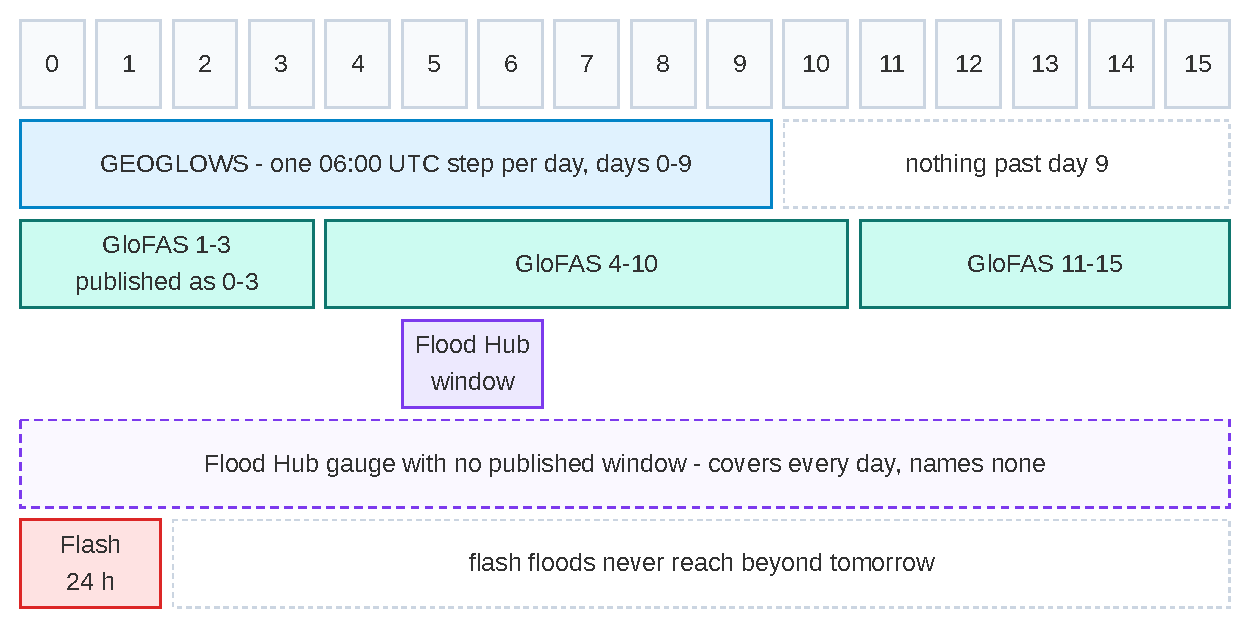
\includegraphics[width=\textwidth]{figures/forecast-timeline.pdf}
\caption[How each model reports a forecast day]{%
  \textbf{What each model means by a forecast day.}
  One column per forecast day, one row per model.
  A \textbf{solid} block names the days it covers, so it earns those days a
  place on the timeline. A \textbf{dashed} block covers days without naming
  any: it is drawn on each of them, but cannot by itself make a day worth
  stepping to. Colour here separates the models in the diagram only --- on the
  map they share a palette and are told apart by the panel.}
\label{fig:forecast-timeline}
\end{figure}
